\section{Attack}\label{sec:attack}

\begin{figure}[t]
	\centering
	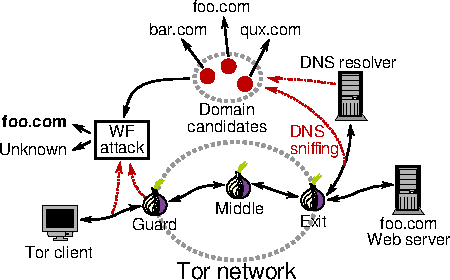
\includegraphics[width=\linewidth]{figures/attack-scenario.pdf}
	\caption{An overview of our correlation attack.  Ingress traffic is
	monitored either by a network-level adversary or the guard relay.  Egress
	traffic is monitored either by a network-level adversary or a DNS server.
	Captured DNS queries then serve as the candidate set for a Website
	fingerprinting attack.}
	\label{fig:attack-scenario}
\end{figure}

Our attack is illustrated in Figure~\ref{fig:attack-scenario} and requires the
following building blocks:
\begin{description}
	\item[Ingress sniffing] An attacker must observe traffic that is entering
		the Tor network.  The attacker can operate on the network level, i.e.,
		be a malicious ISP, or an intelligence agency.  In addition, the
		attacker can operate on the relay level, i.e., run a malicious Tor guard
		relay.  Note that in both cases, the attacker can only observe encrypted
		data.  Therefore, packet meta information such as packet lengths and
		directions serve as input to a website fingerprinting
		attack~\cite{Panchenko2016a}.
	\item[Egress sniffing] To observe both ends of the communication, an
		attacker must also observe egress DNS traffic.  We expect the adversary
		to operate on the network level, i.e., be on the path between exit relay
		and a DNS server.  Alternatively, the attacker can run a malicious DNS
		resolver or server.  Note that an attacker may also run an exit relay,
		but in that case she might as well do classical end-to-end correlation.
	\item[WF fingerprinting] We employ a website fingerprinting attack to
		determine if any of the recently observed DNS queries in egress traffic
		could be part of the encrypted ingress traffic.  Note that the DNS query
		itself does not tell us what \emph{page} a user is going to.
\end{description}

\subsection{Egress sniffing}

How many DNS requests does an exit relay see in $n$ minutes?
\begin{itemize}
	\item We can measure request frequency \emph{without} capturing payload.
	\item We further reduce noise by taking timestamp modulo $m$.
	\item We can do this on an exit relay, or on the DNS root.
	\item \texttt{tshark -f 'udp port 53' -T fields -e frame.time\_epoch -Y 'dns.qry.type == 1 and dns.flags.response == 0'}
	\item Number of requests probably depends on current bandwidth load (which
		we can obtain from the consensus) and the exit policy (which we can
		obtain from the descriptor).
	\item We can limit our exit policy to 80 and 443, so we have a decent
		baseline for requests caused by web traffic.
	\item Fetch relayed traffic from descriptors and use it to normalise
		observed DNS requests.
\end{itemize}

\subsection{Website fingerprinting}
We have to overcome the following problems:
\begin{itemize}
	\item DNS sniffing only tells us what \emph{domains}, but not what
		\emph{pages} a user visits.  Can be a big problem, e.g., with Wikipedia.
	\item DNS records are cached by the resolver for the duration of the TTL.
\end{itemize}

The following aspects might work in our favor:
\begin{itemize}
	\item When visiting a page, your browser sends \emph{multiple} DNS queries.
	\item In tor, the DNS cache enforces a minimum TTL of 60 seconds and a maximum
	TTL of 30 minutes (see tor/src/or/dns.c:278).
\end{itemize}

We gathered five samples of Alexa top 10,000 sites using Firefox 38.7.1 ESR
configured like TBB 5.5.4 and recorded all DNS requests and responses.
We found 59,842 unique domains that only appear on one site, with the per site
number of unique domains mean 6, std 5.6, median 4, min 0, and max 118.
98.2\% out of all sites have unique domains.
Figure~\ref{fig:dns-unique-domains-ff} shows the distribution of sites
without unique domains. Primarily sites in the top 100 of Alexa lacks unique
domains. Applying the Tor cache enforced minimum and maxium TTL, the unique
domain minimum TTL for each site with unique domains have mean 353.6, std 522.0,
median 60, min 60, and max 1800. In other words: for half of the sites in
Alexa top-10,000, there is at least one unique domain with TTL 60 seconds.
This means that if the site has not been requested within the last minute
by a tor exit then the tor exit will send at least one DNS request containing
a uniquely identifying domain for half of the sites in Alexa top-10,000.

\begin{figure}[t]
	\centering
	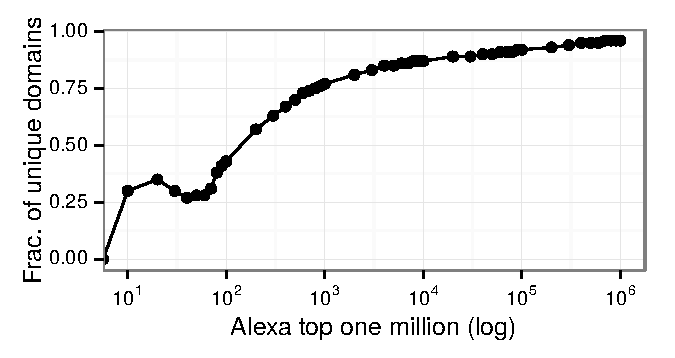
\includegraphics[width=\linewidth]{figures/dns-unique-domains}
	\caption{The distribution of site on Alexa top 10,000 without unique domains.
	Gathered March 25-27 2016 with five samples.}
	\label{fig:dns-unique-domains-ff}
\end{figure}

Other facts that are relevant here:
\begin{itemize}
	\item Tor Browser does not prefetch domain names, but content providers can
	make Tor Browser resolve arbitrary domains by including images or scripts
	with sources of their choice into pages. 
\end{itemize}
